\documentclass{beamer}
\usetheme{Frankfurt}
\usecolortheme{dove}
\newenvironment{alltt}{\ttfamily}{\par}
\usepackage{amsmath,amssymb,amsfonts,amsthm, multicol, subfigure, color}
\usepackage{bm}
\usepackage{graphicx}
\usepackage{hyperref}
\usepackage{pdfpages}
\definecolor{dodgerblue}{rgb}{.118, .575, 1}
\def\independenT#1#2{\mathrel{\rlap{$#1#2$}\mkern2mu{#1#2}}}
\newcommand\independent{\protect\mathpalette{\protect\independenT}{\perp}}
\newcommand\indep{\protect\mathpalette{\protect\independenT}{\perp}}
\def\logit{\text{logit}}
\usepackage{stackrel}
\usepackage{tikz}
\usetikzlibrary{arrows,shapes.arrows,positioning,shapes}
\newcommand\red[1]{{\color{red}#1}}
\newcommand\blue[1]{{\color{blue}#1}}
\newcommand\bblue[1]{{\color{blue}\textbf{#1}}}
\newcommand\green[1]{{\color{olive}#1}}
\newcommand\bgreen[1]{{\color{olive}\textbf{#1}}}
\newcommand\purple[1]{{\color{purple}#1}}
\newcommand\orange[1]{{\color{orange}#1}}
\newcommand\black[1]{{\color{black}#1}}
\newcommand\white[1]{{\color{white}#1}}
\newcommand\teal[1]{{\color{teal}#1}}
\newcommand\magenta[1]{{\color{magenta}#1}}
\newcommand\Fuchsia[1]{{\color{Fuchsia}#1}}
\newcommand\BlueGreen[1]{{\color{BlueGreen}#1}}
\newcommand\iid{\stackrel{\text{iid}}{\sim}}
\newcommand\E{\text{E}}

\title{\blue{Precept 6: Duration models}}
\subtitle{\green{Soc 504: Advanced Social Statistics}}
\author{Ian Lundberg}
\institute[Princeton]{Princeton University}
\date{March 16, 2018}

\begin{document}

\frame{\titlepage}

\begin{frame}
\frametitle{Outline}
\tableofcontents
\end{frame}

\section{Workflow}

\begin{frame}
We've gotten some questions about our personal project workflows. \vskip .2cm
\bblue{Rmarkdown} is in some ways ideal:
\begin{itemize}
\item Fully reproducible
\item Code and results in one place
\end{itemize}
\bgreen{Problem:} If code is slow to run, Rmarkdown is slow to compile each time. \vskip .5cm
I more often use \bblue{R} and \blue{\LaTeX}:
\begin{itemize}
\item In RStudio, you can create a new R script. This is your code but does not produce a PDF.
\item Save results (see \href{https://stat.ethz.ch/R-manual/R-devel/library/base/html/save.html}{\blue{?save}}, \href{http://ggplot2.tidyverse.org/reference/ggsave.html}{\blue{ggsave}}, etc.)
\item Produce final report in \LaTeX
\begin{itemize}
\item I use \blue{\href{http://pages.uoregon.edu/koch/texshop/}{TexShop}}
\item You can also work in an online platform like \blue{\href{https://www.overleaf.com/}{Overleaf}}.\\They also provide great \href{https://www.overleaf.com/latex/templates}{\blue{templates}}!
\end{itemize}
\end{itemize}

\end{frame}

\section{Duration}

\begin{frame}
\frametitle{Outline}
\tableofcontents[currentsection]
\end{frame}

\begin{frame}
\bgreen{Duration models} are useful when we are interested in the
\begin{center}
\large \bblue{time $T$ to an event}
\end{center}
but some observations are \bblue{censored}: the event has not occurred at the end of data collection 
\vskip .5cm
\bblue{Think, pair, share:} \\
Why can't we do OLS when some observations are censored? \pause
Because for those observations we don't know $T$!
\end{frame}

\begin{frame}
The time to death $T$ is a random variable. \\
Its distribution is described by \blue{four critical functions}: \vskip .2cm
1. \bgreen{Density function} $f(t)$ \\
\begin{itemize}
\item Density of death at $t$
\end{itemize}
2. \bgreen{CDF} $F(t) = P(T < t)$ \\
\begin{itemize}
\item Probability of death by $t$
\end{itemize}
3. \bgreen{Survival function} $S(t) = P(T > t) = 1 - F(t)$ \\
\begin{itemize}
\item Probability of survival to $t$
\end{itemize}
4. \bgreen{Hazard function} $h(t) = \frac{f(t)}{S(t)}$
\begin{itemize}
\item Density of death at $t$ given survival up to $t$
\end{itemize} \vskip .5cm
\bblue{Question:} Why isn't the hazard function a probability?
\end{frame}

\begin{frame}

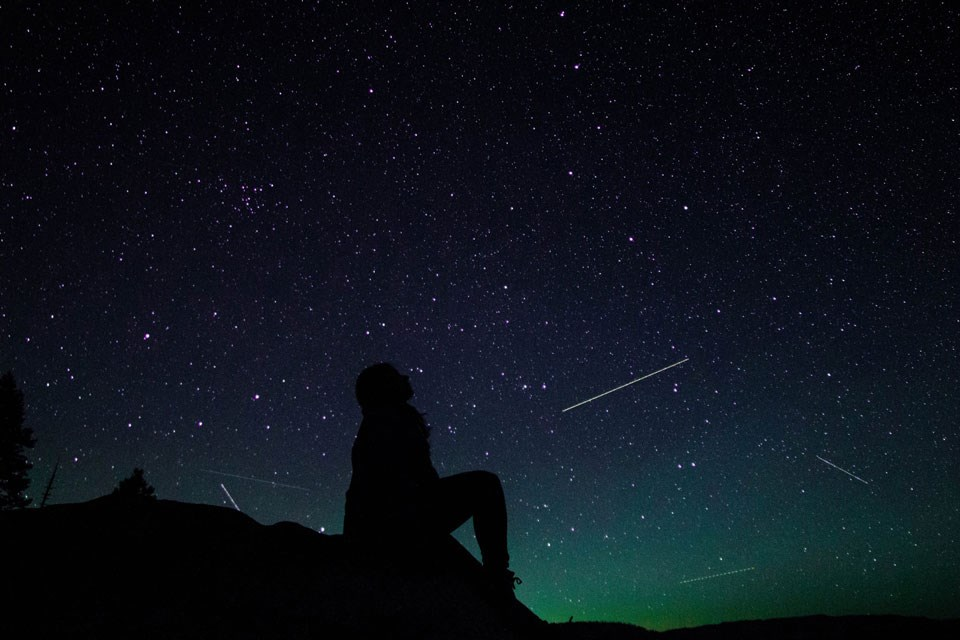
\includegraphics[width = \textwidth]{figs/stargazing} \\
\footnotesize Photo credit: J Zamudio via \url{https://www.nps.gov/yose/planyourvisit/stargazing.htm}

\end{frame}

\begin{frame}{Exponential distribution $\blue{T\sim \text{Exponential}(\lambda)}$}
\bgreen{PDF}
$$f(t) = \lambda e^{-\lambda t}$$
\bgreen{CDF}
$$F(t) = 1 - e^{-\lambda t}$$
\bgreen{Survival function}
$$S(t) = \pause P(T > t) = \pause 1 - P(T<t) = \pause 1 - F_T(t) = \pause e^{-\lambda t}$$
\bgreen{Hazard function:} \pause
$$h(t) = \pause \frac{f(t)}{S(t)} = \pause \frac{\lambda e^{-\lambda t}}{\pause e^{-\lambda t}} = \pause \lambda$$ \pause
We just proved the memoryless property! \bblue{How?} \\ \pause
$h(t)$ is not a function of $t$. The hazard is \bgreen{constant}.
\end{frame}

\begin{frame}{Modeling with covariates}
Suppose we want to allow the hazard to vary by some set of predictors. \vskip .5cm \pause
Then, we can assume a \bblue{proportional hazards} model.\vskip .5cm \pause
\begin{center}
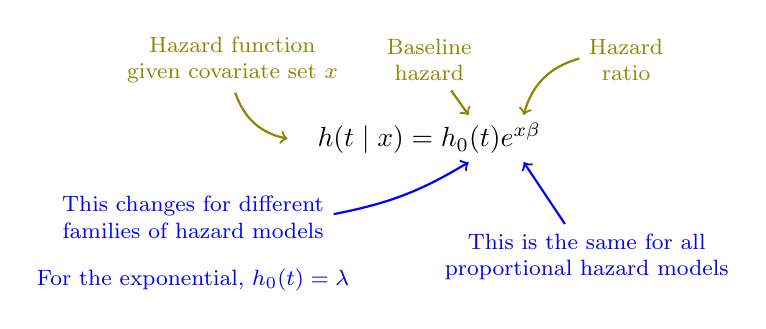
\begin{tikzpicture}
\node at (0,0) {$h(t\mid x) = h_0(t)e^{x\beta}$};
\onslide<4->{
\node[align=center,font=\footnotesize,olive] at (-2.5,1) (h) {Hazard function\\given covariate set $x$};
\node[align=center,font=\footnotesize,olive] at (0,1) (h0) {Baseline\\hazard};
\node[align=center,font=\footnotesize,olive] at (2.5,1) (hr) {Hazard\\ratio};
\draw[->, thick, olive] (h) to[bend right] (-1.8,0);
\draw[->, thick, olive] (h0) -- (.5,0.3);
\draw[->, thick, olive] (hr) to[bend right] (1.2,.3);
}
\onslide<5->{
\node[align=center,font=\footnotesize,blue] at (-3,-1) (changes) {This changes for different\\families of hazard models};
\draw[->, thick, blue] (changes) to[bend right = 10] (.5,-.3);
}
\onslide<6->{
\node[align=center,font=\footnotesize,blue] at (2,-1.5) (same) {This is the same for all\\proportional hazard models};
\draw[->, thick, blue] (same) -- (1.2,-.3);
}
\onslide<7->{
\node[align=center,font=\footnotesize,blue] at (-3,-1.8) (lambda) {For the exponential, $h_0(t) = \lambda$};
}
\end{tikzpicture}
\end{center}
\end{frame}

\begin{frame}{Why add covariates? \pause It might be cloudy.}
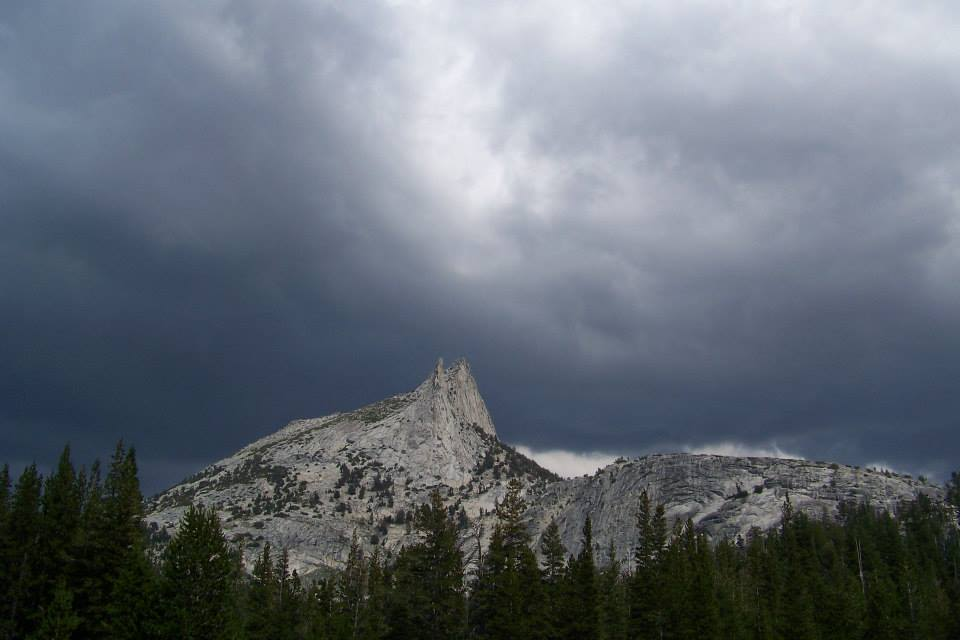
\includegraphics[width = .9\textwidth]{figs/tuolumne_clouds} \\
\footnotesize Photo credit: Hannah Lundberg
\end{frame}

\begin{frame}{Exponential hazards}
\centering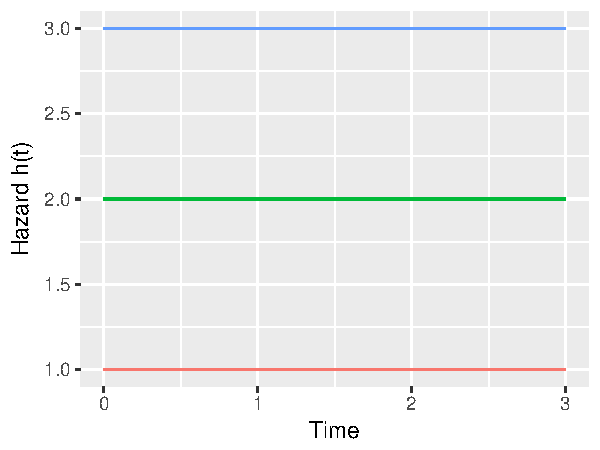
\includegraphics[width = .8\textwidth]{figs/ExpoHazards} \vskip .2cm
\bblue{Question:} If the \green{green} is the baseline hazard $h_0(t)$, what is the hazard ratio that produces the \blue{blue} line? The \red{red} line?
\end{frame}

\begin{frame}[fragile]{Fitting an Exponential with \texttt{survreg}}
\begin{footnotesize}
\begin{semiverbatim}
> library(survival)
> fit <- survreg(Surv(time, event) ~ age + sex,
+                dist = "exponential",
+                data = lung)
> summary(fit)

Call:
survreg(formula = Surv(time, event) ~ age + sex, data = lung, 
    dist = "exponential")
              Value Std. Error     z        p
(Intercept)  6.3597    0.63547 10.01 1.41e-23
age         -0.0156    0.00911 -1.72 8.63e-02
sex          0.4809    0.16709  2.88 4.00e-03

Exponential distribution
Loglik(model)= -1156.1   Loglik(intercept only)= -1162.3
	Chisq= 12.48 on 2 degrees of freedom, p= 0.002 
Number of Newton-Raphson Iterations: 4 
n= 228 
\end{semiverbatim}
\end{footnotesize}
\end{frame}

\begin{frame}[fragile]{Interpreting hazard ratios}
$$h(t\mid x) = h_0(t)e^{-x\beta}$$
\begin{semiverbatim}
> exp(-coef(fit))
(Intercept)         age         sex 
      0.002       1.016       0.618
\end{semiverbatim}
\bblue{Q:} How would you interpret these? \\ \pause
A year increase in age is associated with a 1.6\% increase in the hazard, holding sex constant.
\end{frame}

\begin{frame}
\large
There are some things demographers just memorize. \vskip .5cm
We recommend just looking these up when you need them. \vskip .5cm
For instance, this fact: \vskip .5cm
\begin{center}
\blue{The survival function is e to the minus cumulative hazard.}
\end{center}
\end{frame}

\begin{frame}{Hazard function $\rightarrow$ survival function}
The derivative of the negative log of the survival function is
\begin{footnotesize}
$$\begin{aligned}
\frac{\partial}{\partial t} \left(-\log\left[S(t)\right]\right) &= \frac{\frac{\partial}{\partial t} \left(-S(t)\right)}{S(t)} \\
&= \frac{\frac{\partial}{\partial t} \left(-[1 - F(t)]\right)}{S(t)} \\
&= \frac{f(t)}{S(t)} = h(t)
\end{aligned}$$
\end{footnotesize} \pause
Doing the reverse, we can go from $h(t)$ to $S(t)$
\begin{footnotesize}
$$\begin{aligned}
\int_0^t \frac{\partial}{\partial t'} \left(-\log\left[S(t')\right]\right)dt &= \int_0^t h(t') dt' \\
-\log\left[S(t)\right] &= \int_0^t h(t') dt' \\
S(t) &= e^{-\int_0^t h(t') dt'}
\end{aligned}$$
\end{footnotesize}
\end{frame}

\begin{frame}{Plotting survival curves}
\centering
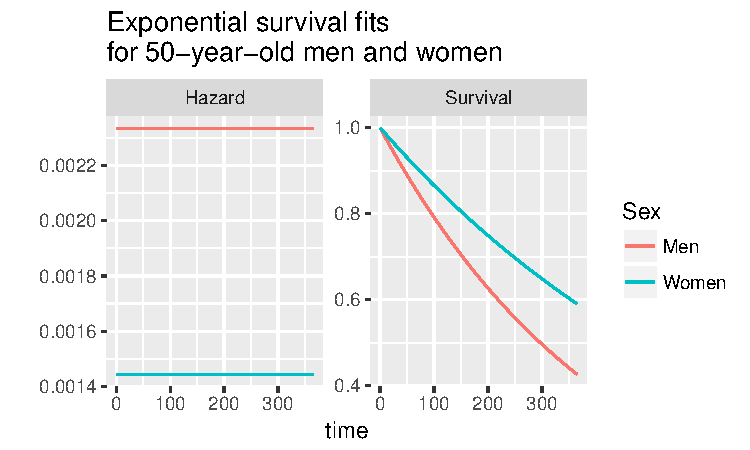
\includegraphics[width = \textwidth]{figs/ExpoFit.pdf}
\end{frame}

\begin{frame}[fragile]{Plotting survival curves}
How we made the previous slide:
\begin{scriptsize}
\begin{semiverbatim}
data.frame(t = seq(.5,20,.5)) %>%
  mutate(Men.Hazard = lambda[1],
         Women.Hazard = lambda[2],
         Men.Survival = exp(-lambda[1]*t),
         Women.Survival = exp(-lambda[2]*t)) %>%
  melt(id = "t") %>%
  separate(variable, into = c("Sex","QOI")) %>%
  ggplot(aes(x = t, y = value, color = Sex)) +
  geom_line() +
  facet_wrap(~QOI, scales = "free") + ylab("") + xlab("time") +
  ggtitle("Exponential survival fits, for 50-year-old men and women") +
  ggsave("ExpoFit.pdf",
         height = 3, width = 5)
\end{semiverbatim}
\end{scriptsize}
\end{frame}

\begin{frame}{Scales and rates}
The exponential is almost always parameterized with a \bblue{rate} $\lambda$. \pause \vskip .5cm
But, it could just as well be defined in terms of a \bblue{scale} $\theta = \frac{1}{\lambda}$ \pause \vskip .5cm
\begin{tabular}{p{.4\textwidth}p{.4\textwidth}}
\bblue{Rate parameterization} & \bblue{Scale parameterization} \\
\hline
\\
$E(T) = \frac{1}{\lambda}$ & $E(T) = \pause \theta$ \\ \pause
$f(T) = \lambda e^{-\lambda x}$ \pause & \pause $f(T) =  \frac{1}{\theta}e^{-\frac{1}{\theta}x}$ \pause \\
As rate grows, expected waiting time shrinks \pause & As scale grows, expected waiting time \pause grows \\
\end{tabular} \vskip .5cm \pause
In general, you have to be careful with the parameterization of survival distributions.
\end{frame}

\begin{frame}
\huge What if we want the hazard to be a function of time? \pause \vskip .5cm \blue{Many options.}
\end{frame}

\begin{frame}{Weibull distribution}
$$T\sim \text{Weibull} (\alpha,\lambda)$$
PDF \footnote{I have used the rate parameterization for $\lambda$; lecture slides use the scale parameterization.}
$$f(t) = t^{\alpha-1}\alpha\lambda^{\alpha} e^{-(\lambda t)^{\alpha}}$$
CDF
$$F(t) = 1 - e^{-(\lambda t)^{\alpha}}$$
Survival function
$$S(t) = P(T > t) = \pause 1 - P(T<t) = \pause 1 - F_T(t) = \pause e^{-(\lambda t)^{\alpha}}$$
Hazard function: \pause Risk of event at $t$ given survival up to $t$ \pause
$$h(t) = \pause \frac{f(t)}{S(t)} = \pause \frac{t^{\alpha-1}\alpha\lambda^{\alpha} e^{-(\lambda t)^{\alpha}}}{\pause e^{-(\lambda t)^{\alpha}}} = \pause t^{\alpha-1}\alpha\lambda^{\alpha}$$
\end{frame}

\begin{frame}{Weibull distribution}
$$h(t) = \frac{f(t)}{S(t)} = \frac{t^{\alpha-1}\alpha\lambda^{\alpha} e^{-(\lambda t)^{\alpha}}}{\pause e^{-(\lambda t)^{\alpha}}} = t^{\alpha-1}\alpha\lambda^{\alpha}$$ \pause \\
The hazard \textcolor{blue}{increases} with $t$ when $\alpha \pause > 1$ \pause \\
The hazard \textcolor{blue}{decreases} with $t$ when $\alpha \pause < 1$ \pause \\
The hazard is \textcolor{blue}{constant} over $t$ when $\alpha \pause = 1$ \pause \\
In that case, it's the exponential! \pause
$$h(t\mid \alpha = 1) = t^{\alpha-1}\alpha\lambda^{\alpha} = t^{1-1}1\lambda^{1} = \lambda$$
\end{frame}

\begin{frame}
\bblue{Discussion:} If the Weibull contains the Exponential as a special case, why not always use the Weibull? \pause \vskip .5cm
The Weibull is more \bgreen{flexible}, which we like. If the world is Weibull but not Exponential, the Weibull is definitely better! \pause \vskip .5cm
If the world is actually Exponential, we gain \bgreen{efficiency} by making the assumption that the hazard is constant over time. \pause \vskip 1cm
This is a \bgreen{general theme} of statistics: Modeling assumptions buy us efficiency if they are correct.
\end{frame}

\begin{frame}{Weibull hazards}
\centering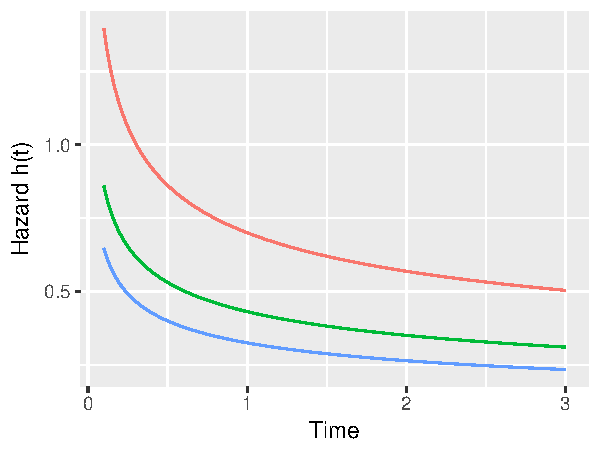
\includegraphics[width = .8\textwidth]{figs/WeibullHazards}
\end{frame}

\begin{frame}[fragile]{Fitting a Weibull model}
\begin{scriptsize}
\begin{semiverbatim}
## Fitting a Weibull model
fit <- survreg(Surv(time, event) ~ age + sex,
               dist = "weibull",
               data = lung)
\end{semiverbatim}
\end{scriptsize}
\end{frame}

\begin{frame}{Weibull results}
\begin{center}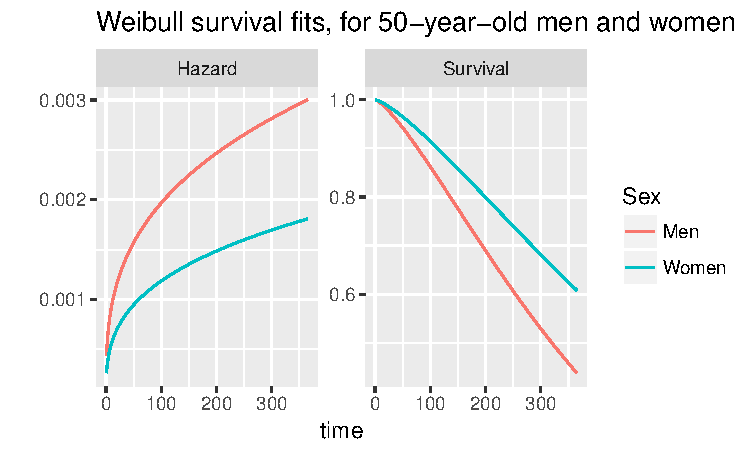
\includegraphics[width = .6\textwidth]{figs/WeibullFit}\end{center}
\bblue{Common question:} The gap between those hazards clearly changes over time! Is this a violation of a modeling assumption? \vskip .2cm \pause
\bblue{A:} No, they are still proportional! \\ \pause
\begin{footnotesize}(Also since these are fitted values, they necessarily agree with the modeling assumptions, so this was a trick question.)\end{footnotesize}
\end{frame}

\begin{frame}
\Large \centering
You can fit a survival model using \\ \bblue{any distribution} \\ for which the support is \\ \bblue{all positive numbers}. \bigskip

There are a huge number of options.

\end{frame}

\begin{frame}{Lognormal distribution}
$$T\sim \text{LogNormal} (\mu,\sigma^2) \sim e^Z\text{ (where }Z\sim N(\mu,\sigma^2)$$
$$f(t) = \frac{1}{Y_i \sigma\sqrt{2\pi}} \text{exp}\left(-\frac{(\ln (Y_i) - \mu)^2}{2\sigma^2}\right)$$
CDF
$$F(t) = \int_0^t f(x) dx = \text{ugly formula}$$
Survival function
$$S(t) = P(T > t) = \pause 1 - P(T<t) = \pause 1 - F_T(t) = \text{ugly formula}$$
Hazard function: \pause Risk of event at $t$ given survival up to $t$ \pause
$$h(t) = \frac{f(t)}{S(t)} = \text{ugly formula}$$
\end{frame}

\begin{frame}[fragile]{Fitting a Lognormal}
\begin{scriptsize}
\begin{semiverbatim}
fit <- survreg(Surv(time, event) ~ age + sex,
               dist = "lognormal",
               data = lung)
\end{semiverbatim}
\end{scriptsize}
Note: This figure doesn't correspond to the model above - just an example of a LogNormal
\begin{center}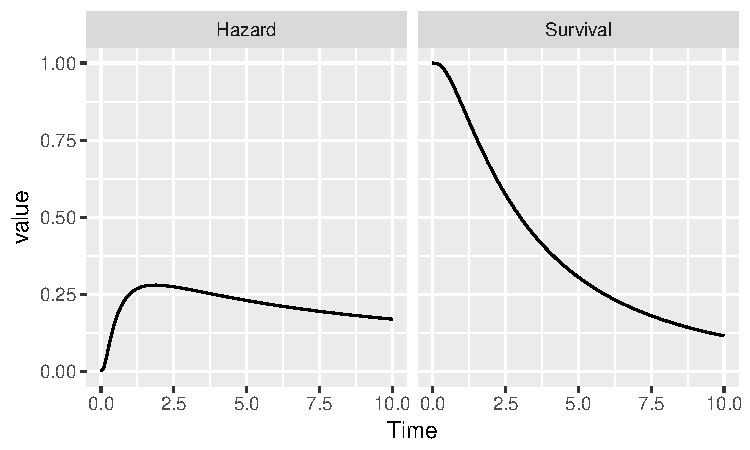
\includegraphics[width = .7\textwidth]{figs/LogNormalExample} \end{center}
\end{frame}

\begin{frame}{Gompertz distribution}
$$\begin{aligned}
f(t) &= b\eta e^{bt}e^\eta \exp(-\eta e^{bt}) \\ \pause
F(t) &= 1-\exp \left(-\eta \left(e^{{bt}}-1\right)\right) \\ \pause
h(t) &= \frac{f(t)}{S(t)} \\ \pause
&= \frac{b\eta e^{bt}e^\eta \exp(-\eta e^{bt})}{\exp \left(-\eta \left(e^{{bt}}-1\right)\right)} \\ \pause
&= b\eta e^{bt}e^\eta \\ \pause
\log[h(t)] &= \underbrace{(\log(b) + \log(\eta) + \eta)}_{\text{Intercept}} + \underbrace{b}_{\text{Slope}}t \\ \pause
&= \alpha + \beta t \\ \pause
\end{aligned}$$ 
The \blue{log of the hazard function} is \green{linear in time!} \\
This is why people like the Gompertz.
\end{frame}

\begin{frame}{Gompertz distribution}
Gompertz hazard with $\alpha = -7, \beta = .09$
$$\log[h(t)] = \alpha + \beta t, \hspace{10pt} h(t) = \exp(\alpha + \beta t)$$ \pause
\bblue{Q:} If the $\log[h(t)]$ increases linearly with $t$, what does $h(t)$ look like?
\begin{center} 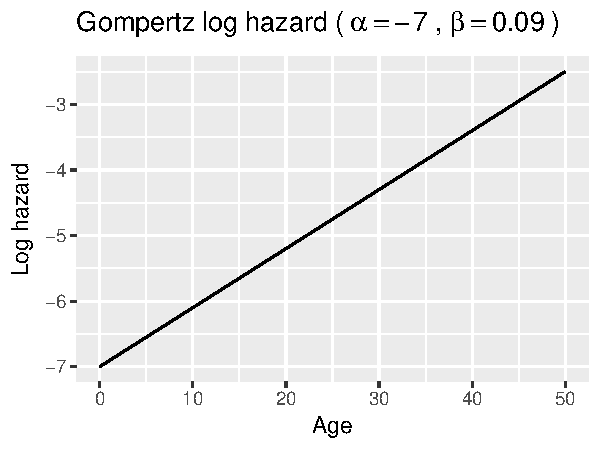
\includegraphics[width = .4\textwidth]{figs/GompertzLogHazard.pdf}\pause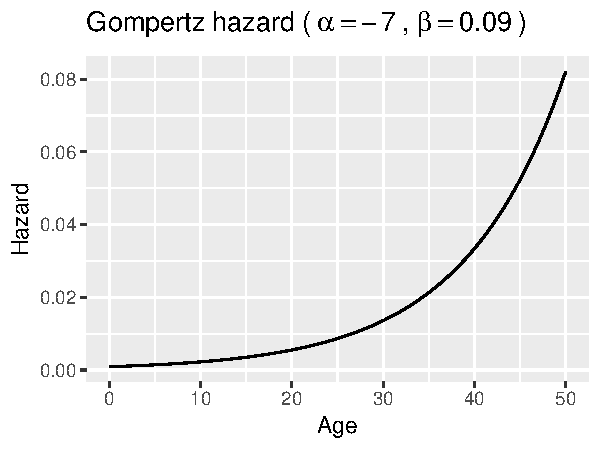
\includegraphics[width = .4\textwidth]{figs/GompertzHazard.pdf} \end{center} \pause
\bblue{Q:} For what questions would this be a good choice? \pause \green{Mortality} \\
\begin{footnotesize}Note: Example motivated by U.S. mortality; see German Rodriguez's \href{http://data.princeton.edu/eco572/us2002gompertz.html}{\textcolor{blue}{example here}}\end{footnotesize}.
\end{frame}

\begin{frame}
\centering
Time between breaks while hiking out of this valley. \\
You don't need a rest right away... \vskip .5cm
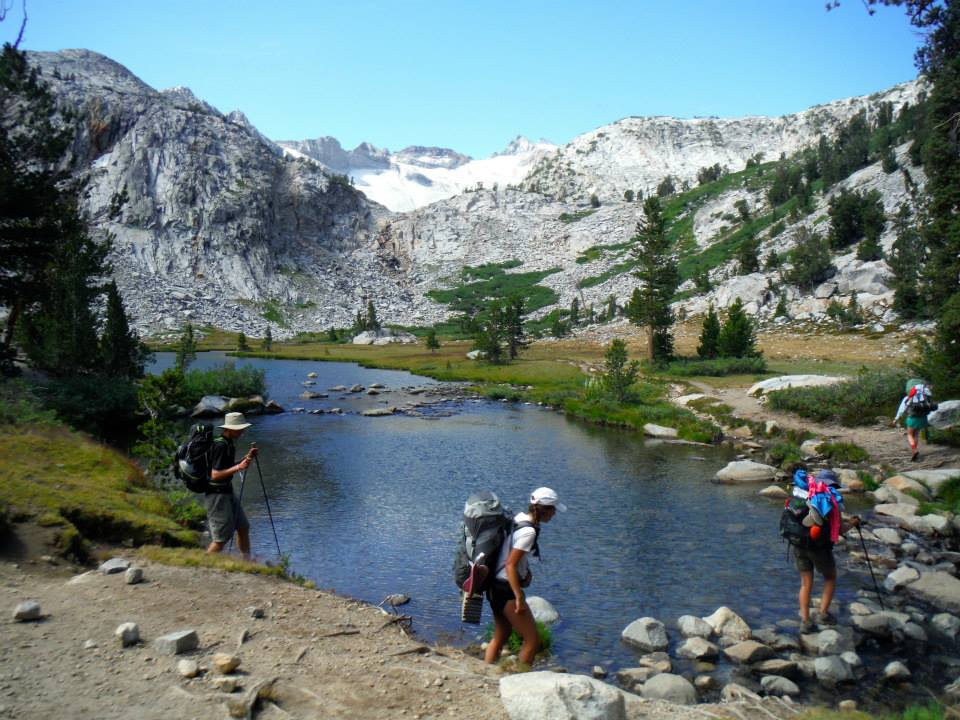
\includegraphics[height = .6\textheight]{figs/donahue_pass} \\
\begin{footnotesize}Donahue Pass, Yosemite. Photo credit: Riley Brian\end{footnotesize}
\end{frame}

\begin{frame}
\centering
...but after going for a while your hazard of resting increases. \\
{\Large \bgreen{Gompertz.}} \vskip .5cm
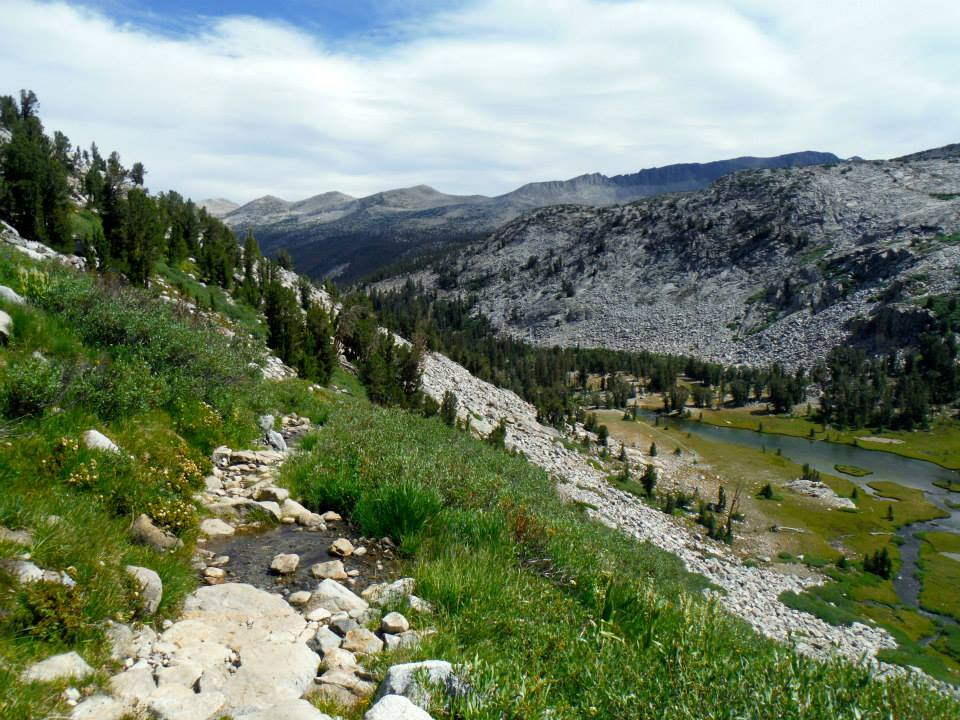
\includegraphics[width = .59\textwidth]{figs/donahue_partway}
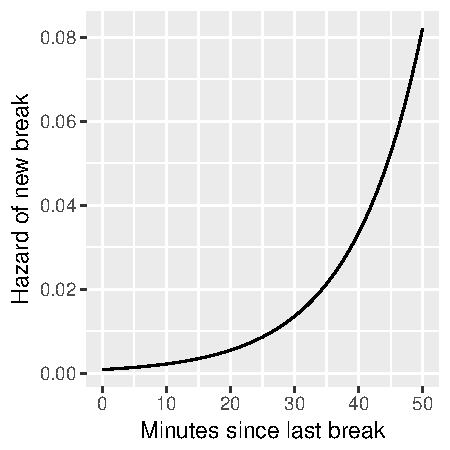
\includegraphics[width = .39\textwidth]{figs/GompertzHazard_hiking.pdf} \\
\begin{flushleft}\begin{footnotesize}Photo credit: Riley Brian\end{footnotesize}\end{flushleft}
\end{frame}

\begin{frame}
As I said at the beginning, \textcolor{blue}{all} of the survival models above have the form:
\begin{center}
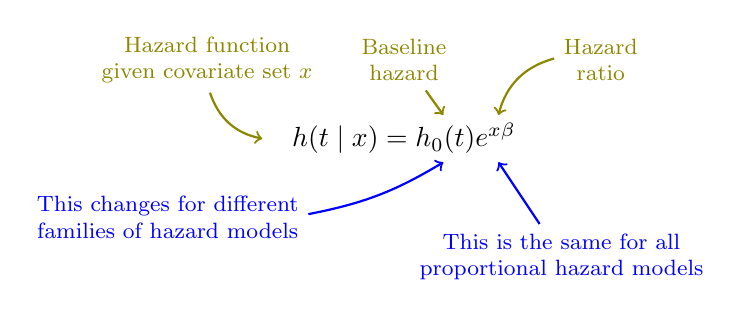
\begin{tikzpicture}
\node at (0,0) {$h(t\mid x) = h_0(t)e^{x\beta}$};
\node[align=center,font=\footnotesize,olive] at (-2.5,1) (h) {Hazard function\\given covariate set $x$};
\node[align=center,font=\footnotesize,olive] at (0,1) (h0) {Baseline\\hazard};
\node[align=center,font=\footnotesize,olive] at (2.5,1) (hr) {Hazard\\ratio};
\draw[->, thick, olive] (h) to[bend right] (-1.8,0);
\draw[->, thick, olive] (h0) -- (.5,0.3);
\draw[->, thick, olive] (hr) to[bend right] (1.2,.3);
\node[align=center,font=\footnotesize,blue] at (-3,-1) (changes) {This changes for different\\families of hazard models};
\draw[->, thick, blue] (changes) to[bend right = 10] (.5,-.3);
\node[align=center,font=\footnotesize,blue] at (2,-1.5) (same) {This is the same for all\\proportional hazard models};
\draw[->, thick, blue] (same) -- (1.2,-.3);
\end{tikzpicture}
\end{center}
%$$S(t) = e^{-\int_0^t h(u) du}$$
Different models allow different kinds of flexibility in the \textcolor{blue}{baseline hazard} $h_0(t)$. \vskip .5cm \pause
Can we model hazard ratios without any assumptions about $h_0(t)$?
\end{frame}

\begin{frame}{Cox proportional hazards model}
Then we can fit a Cox proportional hazards model! \pause \vskip .5cm
To save time, I won't cover this here, but it's important and in lecture slides. \pause \vskip .5cm
The Cox model is fit based on the order at which people die, rather than the times, so it does not assume a baseline hazard. \pause \vskip .5cm
You can fit one with \texttt{coxph()}
\end{frame}

\section{Using distributions}

\begin{frame}
\frametitle{Outline}
\tableofcontents[currentsection]
\end{frame}

\begin{frame}{Using distributions}

\bblue{Most common question we are asked:} \\
How do I know when to use a given distribution for a given problem? \vskip .5cm \pause
When you know the \bgreen{story of the distributions}, you can find one that \bgreen{maps onto} your current problem.

\end{frame}

\begin{frame}{An example we will answer by analogy}
Suppose someone says to you, ``I ran 10 hypothesis tests. What's the probability that the at least 1 $p$-values is less than 0.05 if all the null hypotheses are true?'' \pause \vskip .5cm
You draw this picture. \vskip .5cm
\begin{center}
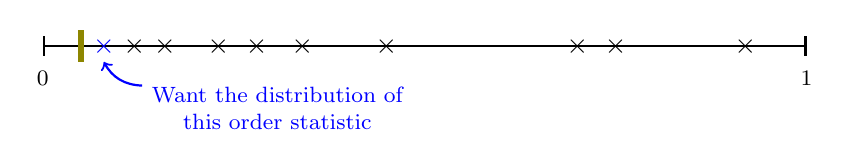
\begin{tikzpicture}[x = .8\textwidth]
\draw[thick,|-|] (0,0) -- (1,0);
\draw[line width = 2pt,olive] (0.05,-.2) -- (0.05, .2);
\node[blue] at (0.08, 0) {$\times$};
\node at (0.12, 0) {$\times$};
\node at (0.16, 0) {$\times$};
\node at (0.23, 0) {$\times$};
\node at (0.28, 0) {$\times$};
\node at (0.34, 0) {$\times$};
\node at (0.45, 0) {$\times$};
\node at (0.70, 0) {$\times$};
\node at (0.75, 0) {$\times$};
\node at (0.92, 0) {$\times$};
\node[anchor = north, font = \footnotesize] at (0,-.2) {0};
\node[anchor = north, font = \footnotesize] at (1,-.2) {1};
\onslide<2->{
\draw[->, thick, blue] (0.13, -.5) to[bend left] (0.08, -.2);
\node[anchor = north west, blue, font = \footnotesize, align = center] at (0.13, -.4) {Want the distribution of\\this order statistic};
}
\end{tikzpicture}
\end{center} \pause
You reply: \\
``You want to know the distribution of the \blue{order statistic $U_{(3)}$}. \pause \\
Let me take you to the wilderness. We will count shooting stars.''
\end{frame}

\begin{frame}
%I'd like to take you to the wilderness of the Sierra Nevada mountains, to one of my favorite places: Rae Lakes.
\begin{center}
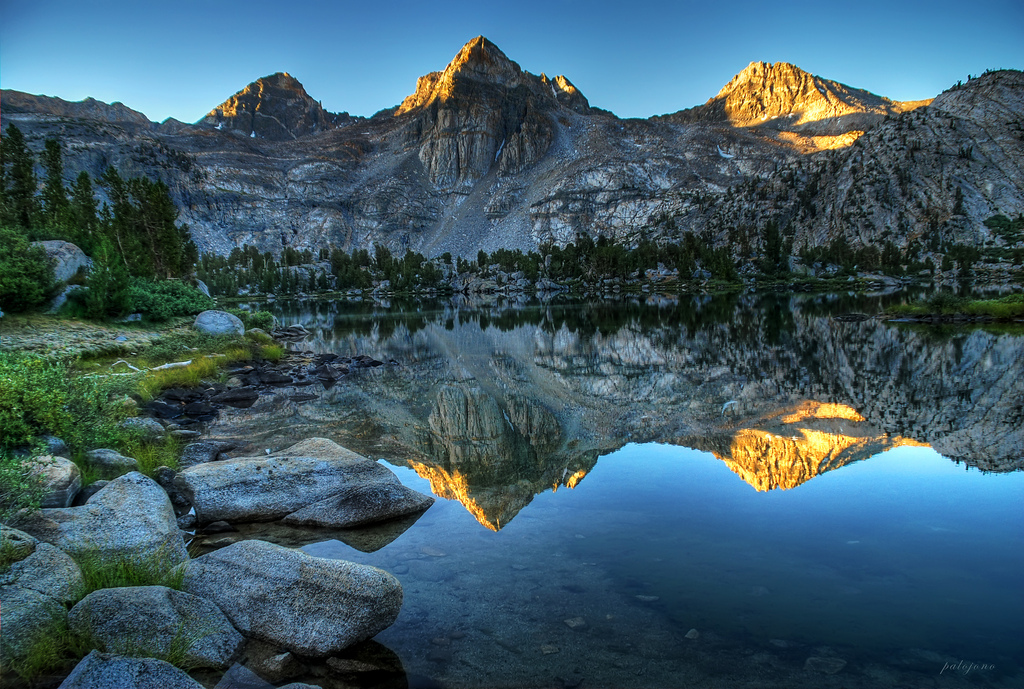
\includegraphics[width = \textwidth]{figs/RaeLakes} \\
\begin{footnotesize}PC: \url{http://wilderness.org/30-prettiest-lakes-wildlands}\end{footnotesize}
\end{center}
\end{frame}

\begin{frame}
Imagine laying out on your pad on the granite, looking up at the sky. \vskip .5cm
We will count shooting stars and record the times we see them.\footnote{Thanks to William Chen for the shooting stars example. See more at \url{http://www.wzchen.com/probability-cheatsheet/}.}
\begin{center}
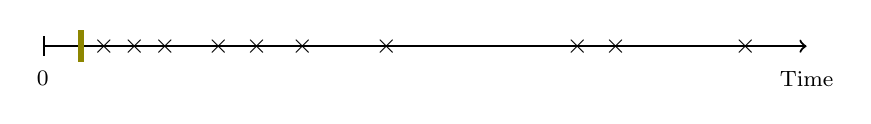
\begin{tikzpicture}[x = .8\textwidth]
\draw[thick,|->] (0,0) -- (1,0);
\draw[line width = 2pt,olive] (0.05,-.2) -- (0.05, .2);
\onslide<2->{\node at (0.08, 0) {$\times$};}
\onslide<3->{\node at (0.12, 0) {$\times$};}
\onslide<4->{\node at (0.16, 0) {$\times$};}
\onslide<5->{\node at (0.23, 0) {$\times$};}
\onslide<6->{\node at (0.28, 0) {$\times$};}
\onslide<7->{\node at (0.34, 0) {$\times$};}
\onslide<8->{\node at (0.45, 0) {$\times$};}
\onslide<9->{\node at (0.70, 0) {$\times$};}
\onslide<10->{\node at (0.75, 0) {$\times$};}
\onslide<11->{\node at (0.92, 0) {$\times$};}
\node[anchor = north, font = \footnotesize] at (0,-.2) {0};
\node[anchor = north, font = \footnotesize] at (1,-.2) {Time};
\end{tikzpicture}
\end{center}
Shooting stars come at a \bblue{constant rate}. \\
\onslide<12->{The times between the arrivals are $X_1,X_2,\dots \iid \text{Exponential}(\lambda)$.}
\end{frame}

\begin{frame}
Suppose we saw the second star at time $X_1 + X_2 = 1$.\pause \vskip .5cm
\bblue{Q:} What is the distribution of $X_1$ given this information?
\begin{center}\begin{tikzpicture}[x = .5\textwidth]
\draw[thick,|-|] (0,0) -- (1,0);
\node at (0.34, 0) {$\times$};
\node at (0.34, .5) {$X_1$};
\node[anchor = north, font = \footnotesize] at (0,-.2) {0};
\node[anchor = north, font = \footnotesize] at (1,-.2) {$X_1 + X_2 = 1$};
\end{tikzpicture}\end{center} \vskip .5cm
$$\frac{X_1}{X_1 + X_2} \sim \text{Uniform}(0,1) \qquad \pause \leftarrow \text{Same as $p$-value under $H_0$!}$$ \pause \vskip .5cm
\bblue{Q:} If I run one hypothesis test, what is the probability under the null that it falls below 0.05? \pause \vskip .5cm
\bgreen{A:} $P(U < .05) = P\left(\frac{X_1}{X_1 + X_2} < .05\right) = 0.05$
\end{frame}

\begin{frame}
Now suppose we observe $X_1,\dots,X_{11}$ and we rescale so their sum is 1.
\begin{center}
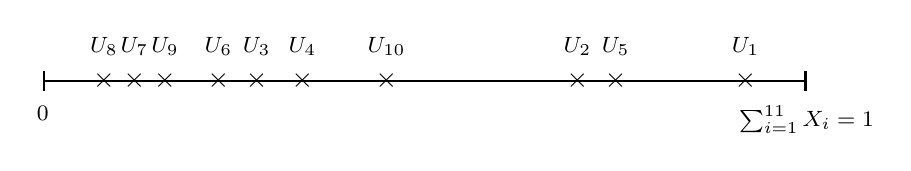
\begin{tikzpicture}[x = .8\textwidth]
\draw[thick,|-|] (0,0) -- (1,0);
%\draw[line width = 2pt,olive] (0.05,-.2) -- (0.05, .2);
\node at (0.08, 0) {$\times$};
\node at (0.12, 0) {$\times$};
\node at (0.16, 0) {$\times$};
\node at (0.23, 0) {$\times$};
\node at (0.28, 0) {$\times$};
\node at (0.34, 0) {$\times$};
\node at (0.45, 0) {$\times$};
\node at (0.70, 0) {$\times$};
\node at (0.75, 0) {$\times$};
\node at (0.92, 0) {$\times$};
\node[font = \footnotesize, anchor = south] at (0.08, .2) {$U_8$};
\node[font = \footnotesize, anchor = south] at (0.12, .2) {$U_7$};
\node[font = \footnotesize, anchor = south] at (0.16, .2) {$U_9$};
\node[font = \footnotesize, anchor = south] at (0.23, .2) {$U_6$};
\node[font = \footnotesize, anchor = south] at (0.28, .2) {$U_3$};
\node[font = \footnotesize, anchor = south] at (0.34, .2) {$U_4$};
\node[font = \footnotesize, anchor = south] at (0.45, .2) {$U_{10}$};
\node[font = \footnotesize, anchor = south] at (0.70, .2) {$U_2$};
\node[font = \footnotesize, anchor = south] at (0.75, .2) {$U_5$};
\node[font = \footnotesize, anchor = south] at (0.92, .2) {$U_1$};
\node[anchor = north, font = \footnotesize] at (0,-.2) {0};
\node[anchor = north, font = \footnotesize] at (1,-.2) {$\sum_{i=1}^{11}X_i = 1$};
\end{tikzpicture}
\end{center}
Let's re-label the $\times$ marks with $U$ values with arbitrary indexes. \vskip .5cm
\bblue{Q:} What is the distribution of the $U_1,\dots,U_{10}$? \\ \pause
\bblue{A:} $U_1,\dots,U_{10}\iid\text{Uniform}(0,1) \quad \leftarrow\text{Same as 10 $p$-values under $H_0$!}$ \pause \vskip .2cm
\begin{center}
\large \blue{There is a connection between $p$-values and shooting stars.}
\end{center}
\end{frame}

\begin{frame}{Order statistics}
\begin{center}
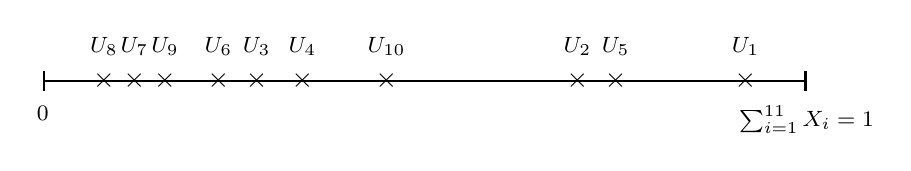
\begin{tikzpicture}[x = .8\textwidth]
\draw[thick,|-|] (0,0) -- (1,0);
%\draw[line width = 2pt,olive] (0.05,-.2) -- (0.05, .2);
\node at (0.08, 0) {$\times$};
\node at (0.12, 0) {$\times$};
\node at (0.16, 0) {$\times$};
\node at (0.23, 0) {$\times$};
\node at (0.28, 0) {$\times$};
\node at (0.34, 0) {$\times$};
\node at (0.45, 0) {$\times$};
\node at (0.70, 0) {$\times$};
\node at (0.75, 0) {$\times$};
\node at (0.92, 0) {$\times$};
\node[font = \footnotesize, anchor = south] at (0.08, .2) {$U_8$};
\node[font = \footnotesize, anchor = south] at (0.12, .2) {$U_7$};
\node[font = \footnotesize, anchor = south] at (0.16, .2) {$U_9$};
\node[font = \footnotesize, anchor = south] at (0.23, .2) {$U_6$};
\node[font = \footnotesize, anchor = south] at (0.28, .2) {$U_3$};
\node[font = \footnotesize, anchor = south] at (0.34, .2) {$U_4$};
\node[font = \footnotesize, anchor = south] at (0.45, .2) {$U_{10}$};
\node[font = \footnotesize, anchor = south] at (0.70, .2) {$U_2$};
\node[font = \footnotesize, anchor = south] at (0.75, .2) {$U_5$};
\node[font = \footnotesize, anchor = south] at (0.92, .2) {$U_1$};
\node[anchor = north, font = \footnotesize] at (0,-.2) {0};
\node[anchor = north, font = \footnotesize] at (1,-.2) {$\sum_{i=1}^{11}X_i = 1$};
\end{tikzpicture}
\end{center}
\large Let's denote the $k$-th \blue{order statistic} by $U_{(k)}$.
\begin{center}
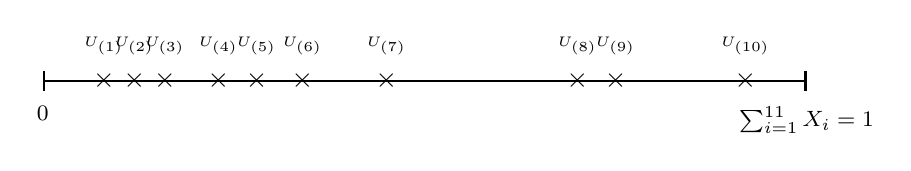
\begin{tikzpicture}[x = .8\textwidth]
\draw[thick,|-|] (0,0) -- (1,0);
%\draw[line width = 2pt,olive] (0.05,-.2) -- (0.05, .2);
\node at (0.08, 0) {$\times$};
\node at (0.12, 0) {$\times$};
\node at (0.16, 0) {$\times$};
\node at (0.23, 0) {$\times$};
\node at (0.28, 0) {$\times$};
\node at (0.34, 0) {$\times$};
\node at (0.45, 0) {$\times$};
\node at (0.70, 0) {$\times$};
\node at (0.75, 0) {$\times$};
\node at (0.92, 0) {$\times$};
\node[font = \tiny, anchor = south] at (0.08, .2) {$U_{(1)}$};
\node[font = \tiny, anchor = south] at (0.12, .2) {$U_{(2)}$};
\node[font = \tiny, anchor = south] at (0.16, .2) {$U_{(3)}$};
\node[font = \tiny, anchor = south] at (0.23, .2) {$U_{(4)}$};
\node[font = \tiny, anchor = south] at (0.28, .2) {$U_{(5)}$};
\node[font = \tiny, anchor = south] at (0.34, .2) {$U_{(6)}$};
\node[font = \tiny, anchor = south] at (0.45, .2) {$U_{(7)}$};
\node[font = \tiny, anchor = south] at (0.70, .2) {$U_{(8)}$};
\node[font = \tiny, anchor = south] at (0.75, .2) {$U_{(9)}$};
\node[font = \tiny, anchor = south] at (0.92, .2) {$U_{(10)}$};
\node[anchor = north, font = \footnotesize] at (0,-.2) {0};
\node[anchor = north, font = \footnotesize] at (1,-.2) {$\sum_{i=1}^{11}X_i = 1$};
\end{tikzpicture}
\end{center}
$$U_{(k)} = \frac{\sum_{i=1}^k X_i}{\sum_{i=1}^{11} X_i}$$
\end{frame}

\begin{frame}{A new distribution: The \bblue{Beta}}
If $X_1,\dots,X_n\sim \text{Exponential}$, then $\frac{\sum_{i=1}^k X_i}{\sum_{i=1}^{n} X_i} \sim \text{Beta(k,n - k - 1)}$
\begin{center}
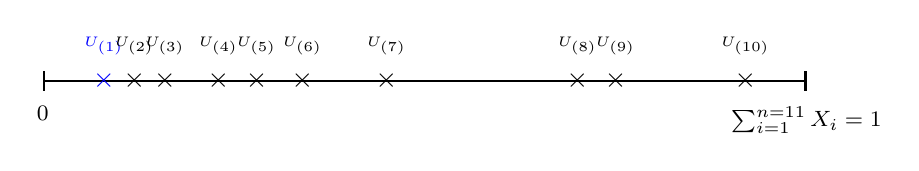
\begin{tikzpicture}[x = .8\textwidth]
\draw[thick,|-|] (0,0) -- (1,0);
%\draw[line width = 2pt,olive] (0.05,-.2) -- (0.05, .2);
\node[blue] at (0.08, 0) {$\times$};
\node at (0.12, 0) {$\times$};
\node at (0.16, 0) {$\times$};
\node at (0.23, 0) {$\times$};
\node at (0.28, 0) {$\times$};
\node at (0.34, 0) {$\times$};
\node at (0.45, 0) {$\times$};
\node at (0.70, 0) {$\times$};
\node at (0.75, 0) {$\times$};
\node at (0.92, 0) {$\times$};
\node[font = \tiny, anchor = south, blue] at (0.08, .2) {$U_{(1)}$};
\node[font = \tiny, anchor = south] at (0.12, .2) {$U_{(2)}$};
\node[font = \tiny, anchor = south] at (0.16, .2) {$U_{(3)}$};
\node[font = \tiny, anchor = south] at (0.23, .2) {$U_{(4)}$};
\node[font = \tiny, anchor = south] at (0.28, .2) {$U_{(5)}$};
\node[font = \tiny, anchor = south] at (0.34, .2) {$U_{(6)}$};
\node[font = \tiny, anchor = south] at (0.45, .2) {$U_{(7)}$};
\node[font = \tiny, anchor = south] at (0.70, .2) {$U_{(8)}$};
\node[font = \tiny, anchor = south] at (0.75, .2) {$U_{(9)}$};
\node[font = \tiny, anchor = south] at (0.92, .2) {$U_{(10)}$};
\node[anchor = north, font = \footnotesize] at (0,-.2) {0};
\node[anchor = north, font = \footnotesize] at (1,-.2) {$\sum_{i=1}^{n = 11}X_i = 1$};
\end{tikzpicture}
\end{center}
So $U_{(1)}\sim \text{Beta}(1,10)$. \vskip .5cm
\bblue{Q:} Can you reason about the expected value of a Beta(1,10)? \vskip .5cm \pause
\bgreen{A:} There are 11 white space that we would expect to be of equal size, so we might expect that $\E(U_{(1)}) = \frac{1}{11}$. \bgreen{This is right!}
\end{frame}

\begin{frame}
\bblue{Q:} Given what we know about shooting stars, what distribution do you think the smallest $p$-value takes?
\begin{center}
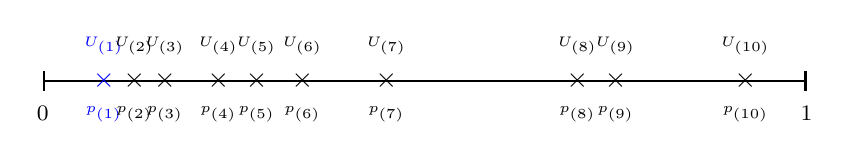
\begin{tikzpicture}[x = .8\textwidth]
\draw[thick,|-|] (0,0) -- (1,0);
%\draw[line width = 2pt,olive] (0.05,-.2) -- (0.05, .2);
\node[blue] at (0.08, 0) {$\times$};
\node at (0.12, 0) {$\times$};
\node at (0.16, 0) {$\times$};
\node at (0.23, 0) {$\times$};
\node at (0.28, 0) {$\times$};
\node at (0.34, 0) {$\times$};
\node at (0.45, 0) {$\times$};
\node at (0.70, 0) {$\times$};
\node at (0.75, 0) {$\times$};
\node at (0.92, 0) {$\times$};
\node[font = \tiny, anchor = south, blue] at (0.08, .2) {$U_{(1)}$};
\node[font = \tiny, anchor = south] at (0.12, .2) {$U_{(2)}$};
\node[font = \tiny, anchor = south] at (0.16, .2) {$U_{(3)}$};
\node[font = \tiny, anchor = south] at (0.23, .2) {$U_{(4)}$};
\node[font = \tiny, anchor = south] at (0.28, .2) {$U_{(5)}$};
\node[font = \tiny, anchor = south] at (0.34, .2) {$U_{(6)}$};
\node[font = \tiny, anchor = south] at (0.45, .2) {$U_{(7)}$};
\node[font = \tiny, anchor = south] at (0.70, .2) {$U_{(8)}$};
\node[font = \tiny, anchor = south] at (0.75, .2) {$U_{(9)}$};
\node[font = \tiny, anchor = south] at (0.92, .2) {$U_{(10)}$};
\node[font = \tiny, anchor = north, blue] at (0.08, -.2) {$p_{(1)}$};
\node[font = \tiny, anchor = north] at (0.12, -.2) {$p_{(2)}$};
\node[font = \tiny, anchor = north] at (0.16, -.2) {$p_{(3)}$};
\node[font = \tiny, anchor = north] at (0.23, -.2) {$p_{(4)}$};
\node[font = \tiny, anchor = north] at (0.28, -.2) {$p_{(5)}$};
\node[font = \tiny, anchor = north] at (0.34, -.2) {$p_{(6)}$};
\node[font = \tiny, anchor = north] at (0.45, -.2) {$p_{(7)}$};
\node[font = \tiny, anchor = north] at (0.70, -.2) {$p_{(8)}$};
\node[font = \tiny, anchor = north] at (0.75, -.2) {$p_{(9)}$};
\node[font = \tiny, anchor = north] at (0.92, -.2) {$p_{(10)}$};
\node[anchor = north, font = \footnotesize] at (0,-.2) {0};
\node[anchor = north, font = \footnotesize] at (1,-.2) {1};
\end{tikzpicture}
\end{center}
\begin{center}\Large \blue{$p_{(1)} \sim \text{Beta}(1,9)$} \end{center}
\bblue{Q:} What is the probability that the smallest $p$-value is less than 0.05?
$$P(p_{(1)} < .05) = P(\text{Beta}(1,10) < .5) = F_{\text{Beta(1,9)}}(.05) = 0.37$$
It is very easy to get a false positive by running 10 hypothesis tests!
\end{frame}

\begin{frame}{Key takeaways}
\begin{columns}
\begin{column}{.5\textwidth}
\Large \centering
We've taught you the\\stories of many distributions. \vskip .5cm
To use them, try to fit your problem into one of these \bblue{known stories}! \vskip .5cm
\end{column}
\begin{column}{.5\textwidth}
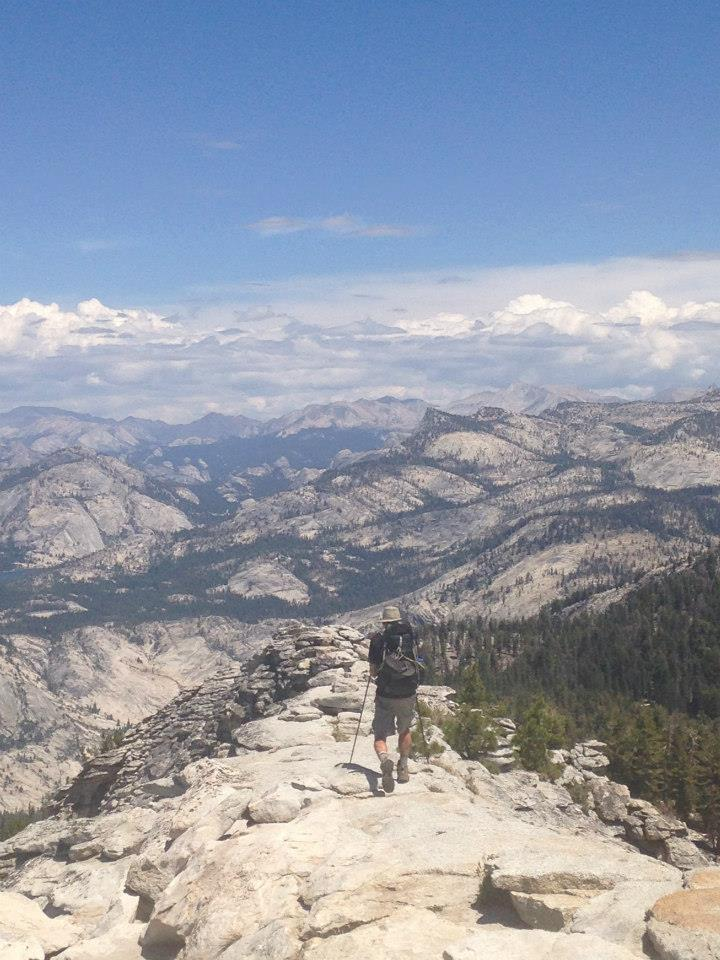
\includegraphics[height = .8\textheight]{figs/clouds_rest} \\
\begin{footnotesize}Photo credit: Hannah Lundberg\end{footnotesize}
\end{column}
\end{columns}
\end{frame}

\begin{frame}
In my own research, I wanted to choose a prior distribution on a correlation that I expected to be near 1. I chose \blue{Beta(3,1)}.
\begin{center}
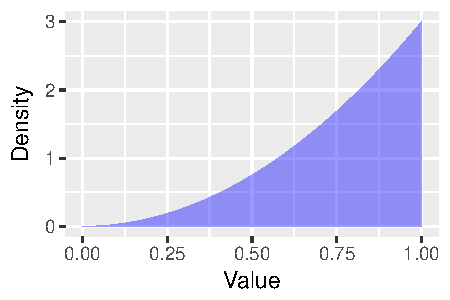
\includegraphics[width = .5\textwidth]{figs/beta_3_1.pdf}
\end{center}
I chose that by thinking:
\begin{itemize}
\item I want the distribution of the highest of 3 uniform draws.
\item I want the distribution of the proportion of time spent waiting for 3 shooting stars, out of a total time spend waiting for 4.
\end{itemize}
\begin{large}Plugging your problem into a \bblue{known story} can help you find a solution.\end{large}
\end{frame}

\begin{frame}{Generalizing that story}
Suppose someone says to you, ``I ran 100 hypothesis tests. What's the probability that the 7th-smallest $p$-value is less than 0.05 if the null hypotheses are true?'' \pause \vskip .5cm

You say...let me take you to the wilderness. We will count shooting stars. \pause \vskip .5cm

That is the proportion of time spent waiting for the 7th shooting star:
$$U_{(7)} \sim \text{Beta}(7,93)$$
$$P(U_{(7)} < .05) = F_{\text{Beta(7,93)}}(.05) = 0.23$$ \pause
So, it's not that strange to see 7 $p$-values less than 0.05. \pause And we learned this all from shooting stars!
\end{frame}

\begin{frame}{One other story you might use}
What if we wanted a distribution for the time until the $k$th star comes?

$$\begin{aligned}
X_1,\dots,X_k &\stackrel{\text{iid}}{\sim} \text{Exponential}(\lambda) \pause \\
G_k &\sim X_1 + \dots + X_k
\end{aligned}$$ \pause
Then we say
$$G_k\sim \text{Gamma}(k,\lambda)$$
The \bblue{Gamma distribution} characterizes the wait time until the $k$th star.
\end{frame}

\section{Zelig}

\begin{frame}
\frametitle{Outline}
\tableofcontents[currentsection]
\end{frame}

\begin{frame}{Side note: Zelig}
Zelig is an R package designed to make everything we do in class easier. \vskip .5cm
Note the Zelig \href{https://github.com/IQSS/Zelig/blob/master/README.md}{\textcolor{blue}{workflow overview}}. \vskip .5cm
We will use the \href{http://docs.zeligproject.org/en/latest/zelig-exp.html}{\textcolor{blue}{Zelig-Exponential}}. \vskip .5cm
\end{frame}

\begin{frame}[fragile]{Zelig example: Lung cancer survival}
We will walk through the example using data on lung cancer survival
\begin{scriptsize}
\begin{semiverbatim}
> library(survival)
> data(lung)
> head(lung)
  inst time status age sex ph.ecog ph.karno pat.karno meal.cal wt.loss
1    3  306      2  74   1       1       90       100     1175      NA
2    3  455      2  68   1       0       90        90     1225      15
3    3 1010      1  56   1       0       90        90       NA      15
4    5  210      2  57   1       1       90        60     1150      11
5    1  883      2  60   1       0      100        90       NA       0
6   12 1022      1  74   1       1       50        80      513       0
lung <- mutate(lung, event = as.numeric(status == 2))
\end{semiverbatim} 
\end{scriptsize}
\end{frame}

\begin{frame}[fragile]{Variable definitions: Lung cancer survival}
\begin{scriptsize}
\begin{semiverbatim}
?lung
inst:	Institution code
time:	Survival time in days
status:	censoring status 1=censored, 2=dead
age:	Age in years
sex:	Male=1 Female=2
ph.ecog:	ECOG performance score (0=good 5=dead)
ph.karno:	Karnofsky performance score (bad=0-good=100) rated by physician
pat.karno:	Karnofsky performance score as rated by patient
meal.cal:	Calories consumed at meals
wt.loss:	Weight loss in last six months
\end{semiverbatim}
\end{scriptsize}
\end{frame}

\begin{frame}[fragile]{Zelig step 1: Fit a model}
\begin{scriptsize}
\begin{semiverbatim}
fit <- zelig(Surv(time, event) ~ age + sex,
             model = "exp",
             data = lung)
\end{semiverbatim}
\end{scriptsize}
\end{frame}

\begin{frame}[fragile]{Zelig step 1: Fit a model}
\begin{scriptsize}
\begin{semiverbatim}
> summary(fit)
Model: 

Call:
z5$zelig(formula = Surv(time, event) ~ age + sex, data = lung)
              Value Std. Error     z        p
(Intercept)  6.3597    0.63547 10.01 1.41e-23
age         -0.0156    0.00911 -1.72 8.63e-02
sex          0.4809    0.16709  2.88 4.00e-03

Scale fixed at 1 

Exponential distribution
Loglik(model)= -1156.1   Loglik(intercept only)= -1162.3
	Chisq= 12.48 on 2 degrees of freedom, p= 0.002 
Number of Newton-Raphson Iterations: 4 
n= 228 

Next step: Use 'setx' method
\end{semiverbatim}
\end{scriptsize}
\end{frame}

\begin{frame}[fragile]{Zelig step 2: Use \texttt{setx} to set covariates of interest}
\begin{scriptsize}
\begin{semiverbatim}
men <- setx(fit, age = 50, sex = 1)
women <- setx(fit, age = 50, sex = 2)
\end{semiverbatim}
\end{scriptsize}
\end{frame}

\begin{frame}[fragile]{Zelig step 2: Use \texttt{setx} to set covariates of interest}
\begin{scriptsize}
\begin{semiverbatim}
> men
setx:
  (Intercept) age sex
1           1  50   1

Next step: Use 'sim' method
> women
setx:
  (Intercept) age sex
1           1  50   2

Next step: Use 'sim' method
\end{semiverbatim}
\end{scriptsize}
\end{frame}

\begin{frame}[fragile]{Zelig step 3: Use \texttt{sim} to simulate quantities of interest}
\begin{tiny}
\begin{semiverbatim}
> sims <- sim(obj = fit, x = men, x1 = women)
> summary(sims)

 sim x :
 -----
ev
     mean       sd      50%     2.5%   97.5%
1 355.086 33.63733 353.5258 296.6169 428.758
pv
        mean       sd     50%     2.5%    97.5%
[1,] 351.414 361.6174 242.511 7.082744 1357.005

 sim x1 :
 -----
ev
      mean      sd     50%     2.5%    97.5%
1 577.5684 78.5113 571.178 438.4341 743.9957
pv
         mean       sd      50%    2.5%   97.5%
[1,] 562.8317 550.6102 382.9658 11.5627 2016.61
fd
      mean      sd      50%     2.5%    97.5%
1 222.4824 85.0493 217.0278 61.08082 396.5632
\end{semiverbatim}
\end{tiny}
\end{frame}

\begin{frame}[fragile]{Zelig step 4: Use \texttt{graph} to plot simulation results}
\begin{scriptsize}
\begin{semiverbatim}
pdf("ZeligFigures.pdf",
    height = 5, width = 7)
plot(sims)
dev.off()
\end{semiverbatim}
\end{scriptsize}
\begin{center}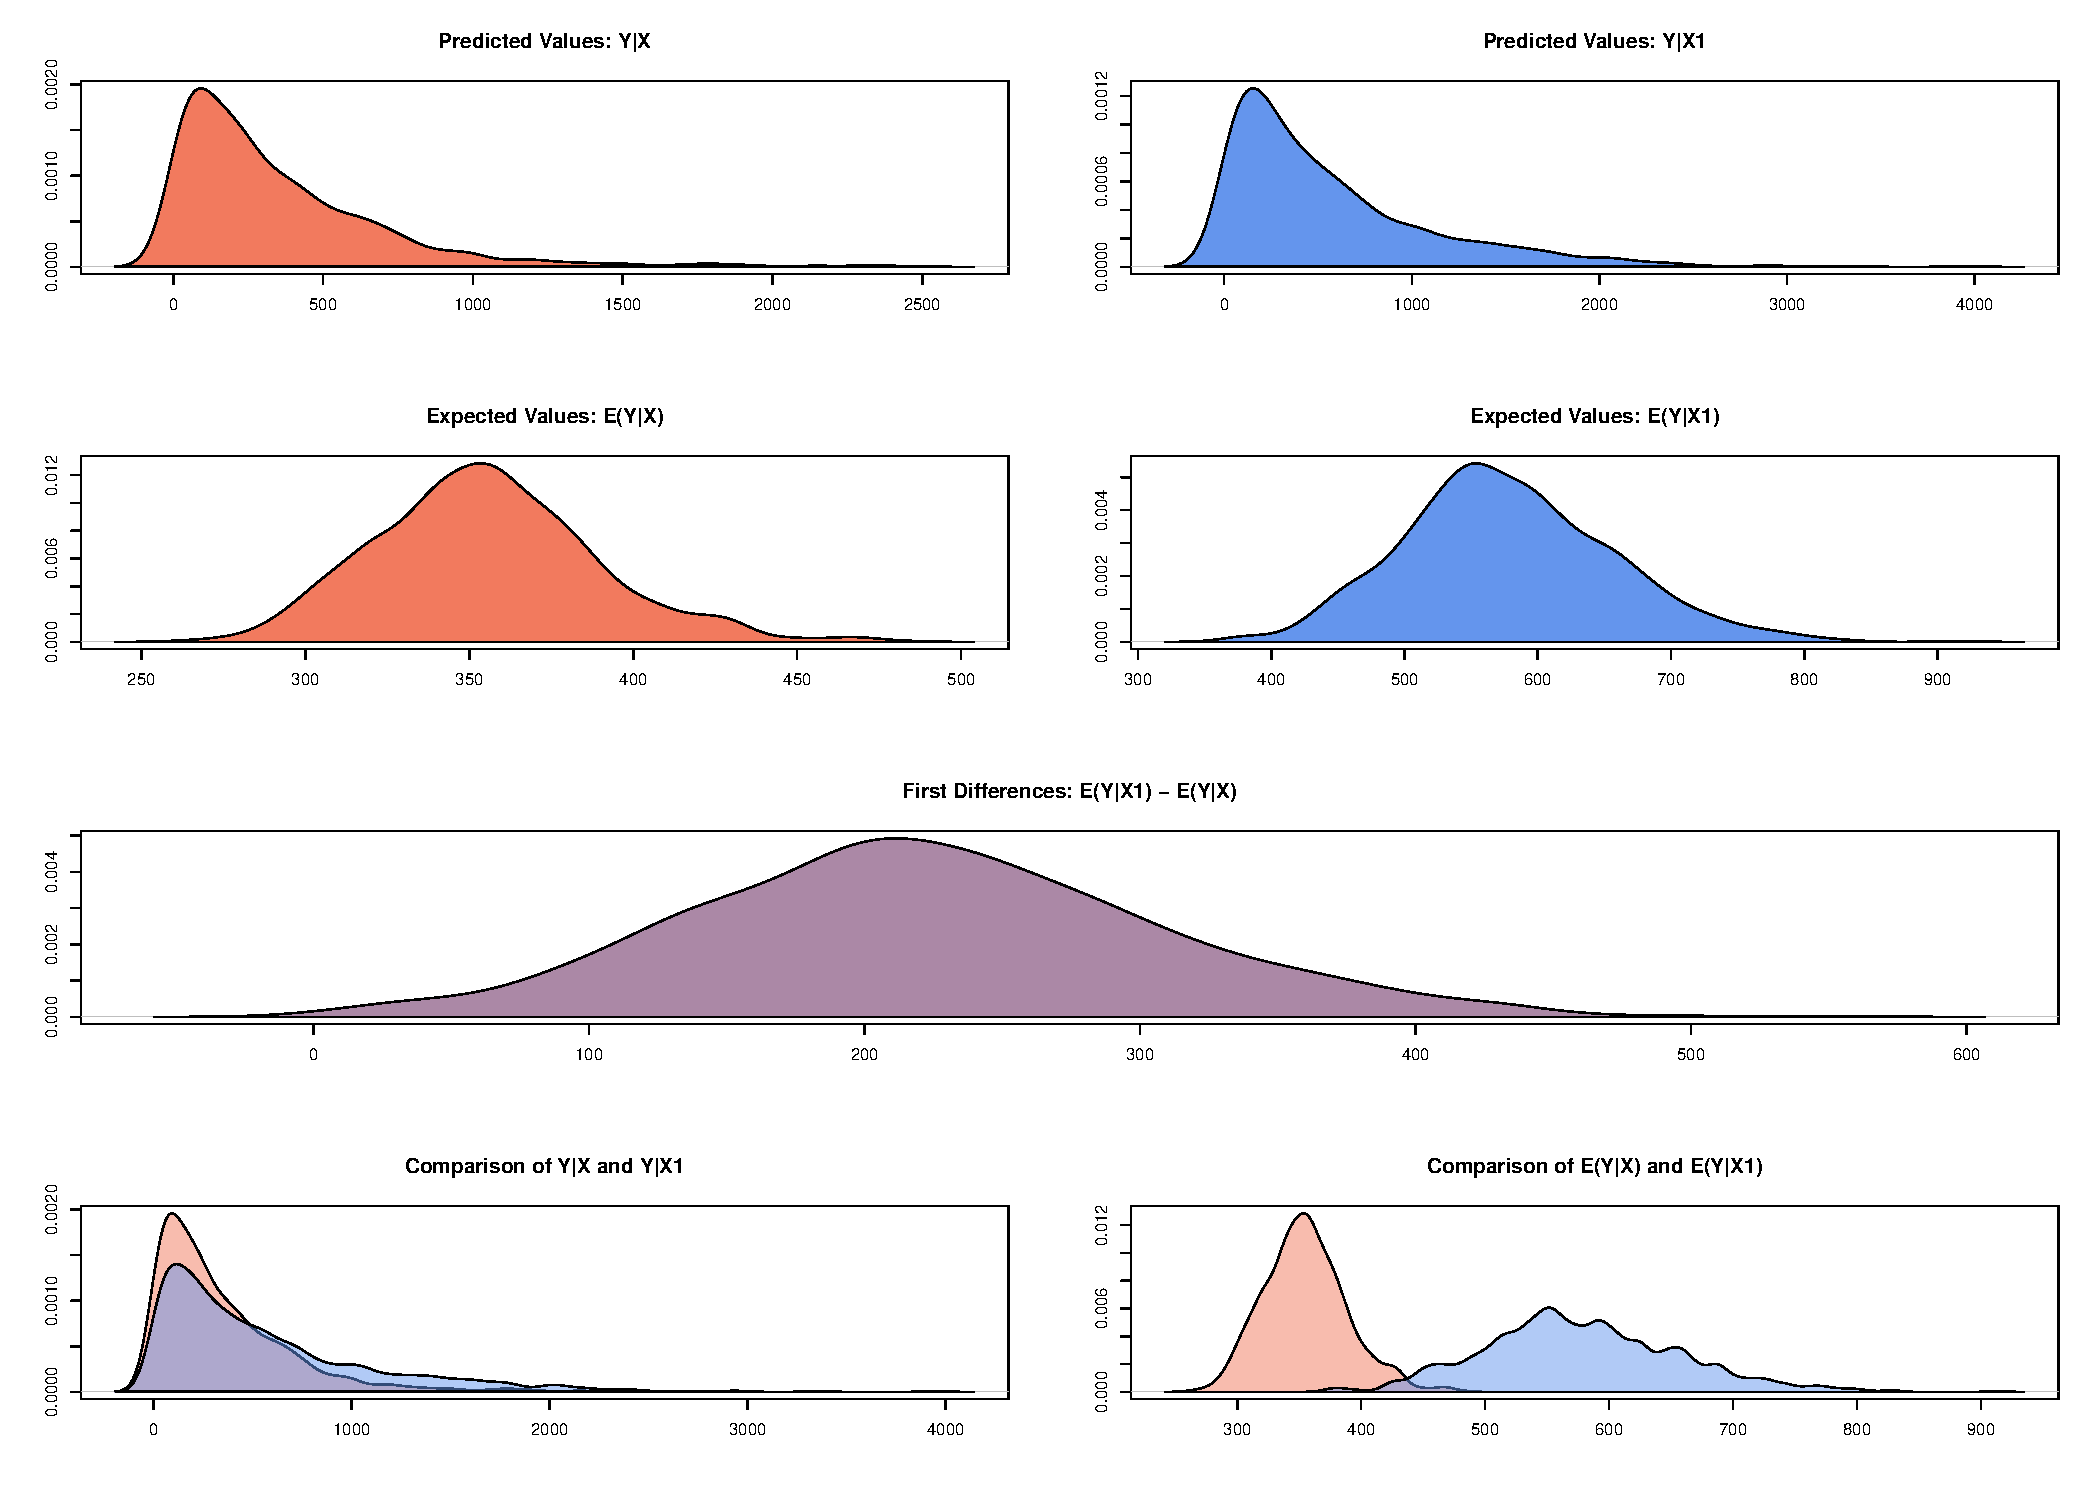
\includegraphics[height = .7\textheight]{figs/ZeligFigures.pdf}\end{center}\footnote{
Note: X = Men, X1 = Women}
\end{frame}

\begin{frame}[fragile]{Summarizing Zelig}
\footnotesize
Estimate your model:\\
\pause
\begin{semiverbatim}
#install.packages("Zelig")
require(Zelig)
fit <- zelig(Surv(time, event) ~ age + sex,
             model = "exp",
             data = lung)
\end{semiverbatim}
\pause
Set your covariates:\\
\pause
\begin{semiverbatim}
men <- setx(fit, sex = 1, fn = mean)
women <- setx(fit, sex = 2, fn = mean)
\end{semiverbatim}
\pause
Simulate your QOI:\\
\pause
\begin{semiverbatim}
sims <- sim(obj = fit, x = men, x1 = women)
\end{semiverbatim}
\pause
Plot:\\ 
\pause
\begin{semiverbatim}
plot(sims)
\end{semiverbatim}
\end{frame}

\begin{frame}
\begin{center}
After break: expectation maximization, missing data
\bigskip \\
\Large \bblue{Cards!} \bgreen{Questions?} \vskip .2cm
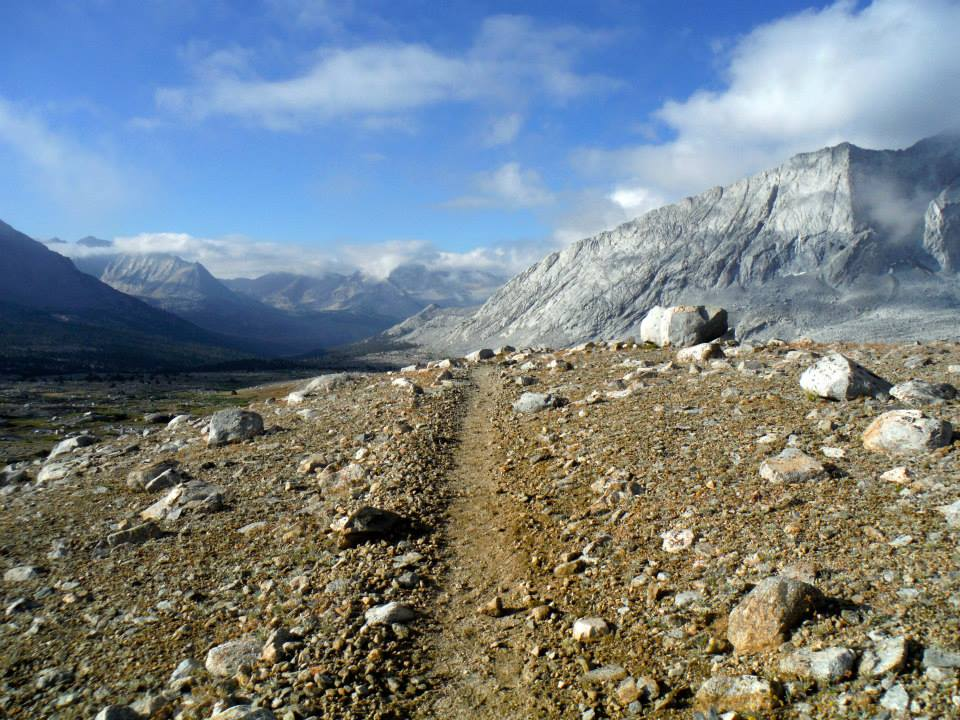
\includegraphics[width = .6\textwidth]{figs/trail} \\
\begin{footnotesize}Photo credit: Riley Brian\end{footnotesize}
\end{center}
\end{frame}



\end{document}
